\uuid{qAIw}
\chapitre{Autre}
\sousChapitre{Autre}
\titre{ Représentation d'une fonction réelle par un réseau de neurones}
\theme{réseaux de neurones}
\auteur{ Maxime NGUYEN }
\datecreate{2024-11-17}
\organisation{ AMSCC }

\contenu{
	
	\question{ 

Concevoir un réseau de neurones qui réalises la fonction $\R \to \R$ suivante :

\begin{center}
	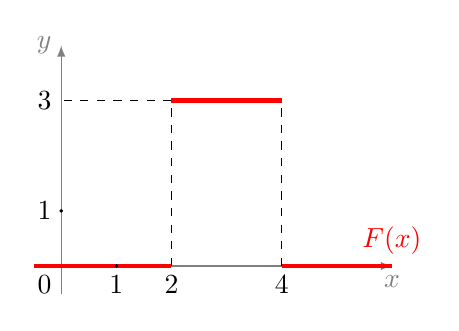
\begin{tikzpicture}[scale=0.7]
	
	\draw[->,>=latex, gray] (-0.5,0)--(6,0) node[below] {$x$};
	\draw[->,>=latex, gray] (0,-0.5)--(0,4) node[left] {$y$};
	
	\draw[ultra thick,red] (-0.5,0) -- (2,0);
	\draw[ultra thick,red] (2,3) -- (4,3);
	
	%\draw[ultra thick,red] (3,0) -- (4,0);
	%\draw[ultra thick,red] (4,2) -- (5,2);
	\draw[ultra thick,red] (4,0) -- (6,0) node[above]{$F(x)$};
	
	\fill[black] (0,1) circle (1pt);
	\fill[black] (1,0) circle (1pt);
	
	\node at (0,0) [below left] {$0$};
	\node at (0,1) [left] {$1$};
	\node at (1,0) [below] {$1$};
	
	\node at (2,0) [below] {$2$};
	%\node at (3,0) [below] {$3$};
	\node at (4,0) [below] {$4$};
	%\node at (5,0) [below] {$5$};
	
	%\draw[dashed] (1,1)--(0,1) node[left]{$1$};
	\draw[dashed] (2,3)--(0,3) node[left]{$3$};
	
	%\draw[dashed] (1,0)--(1,1);
	\draw[dashed] (2,0)--(2,3);
	\draw[dashed] (4,0)--(4,3);
	%\draw[dashed] (5,0)--(5,2);
	
\end{tikzpicture}	
\end{center}
}
}